\documentclass[11pt,letter]{article}
\usepackage{etex}
\usepackage[top=0.65in,bottom=0.9in,left=0.85in,right=0.85in]{geometry}

%\def\baselinestretch{1.25}
%\def\baselinestretch{1.0}

\usepackage[greek, english]{babel}
%\usepackage{multicol}
\usepackage[thinlines]{easytable}

%\usepackage[draft]{graphicx}
\usepackage{graphicx}
\usepackage[export]{adjustbox}

\usepackage{caption}
\usepackage{subcaption}

\usepackage{setspace}
\usepackage{float}

% The use of the times package forces the use of the type-1 times
% roman font, but the times roman font does not look nice.
% Besides the times roman font still does not print correctly on
% the dopy printer.
%\usepackage{times}


\usepackage{fancyhdr}
\usepackage{amsmath}
%\usepackage{amssymb}
\usepackage{bm}
\usepackage{bbold}
\usepackage{parskip}
\usepackage{url}

\usepackage[adobe-utopia]{mathdesign}
\usepackage[T1]{fontenc}

\newcommand{\kb}{\ensuremath{k_{\text{B}}}}

\newcommand{\bv}[1]{\ensuremath{\bm{#1}}}
\newcommand{\Lc}{\ensuremath{L_{\mathrm{c}}}}
\newcommand{\dsig}[1]{\ensuremath{ \frac{ d\,\sigma_{#1} }{d\,\Omega} }}

\newcommand{\isat}{\ensuremath{I_{\mathrm{sat}}}}
\newcommand{\iisat}{\ensuremath{I_{\mathrm{p}}/I_{\mathrm{sat}}}}
\newcommand{\Iqtof}{\ensuremath{I_{\bv{Q}\infty} }}
\newcommand{\Itof}[1]{\ensuremath{I_{\bv{#1}\infty} }}
\newcommand{\Iq}{\ensuremath{I_{\bv{Q}} }}
\newcommand{\iq}{\ensuremath{i_{\bv{Q}} }}
\newcommand{\Iqma}{\ensuremath{I_{\bv{Q}_{\text{MA}}} }}
\newcommand{\Ima}[1]{\ensuremath{I_{\bv{#1}_{\text{MA}}} }}
\newcommand{\iqma}{\ensuremath{i_{\bv{Q}_{\text{MA}}} }}
\newcommand{\jqma}{\ensuremath{j_{\bv{Q}_{\text{MA}}} }}
\newcommand{\Iqmatof}{\ensuremath{I_{\bv{Q}_{\text{MA}\infty}} }}
\newcommand{\is}{\ensuremath{i_{S}} }
\newcommand{\iqT}{\ensuremath{i_{\bv{Q}_{T}} }}
\newcommand{\ipith}{\ensuremath{i_{\bv{\pi}/\bv{\theta}}}}
\newcommand{\fpith}{\ensuremath{f_{\bv{\pi}/\bv{\theta}}}}
\newcommand{\iT}[1]{\ensuremath{i_{\bv{#1}_{T}} }}
\newcommand{\ima}[1]{\ensuremath{i_{\bv{#1}_{\text{MA}}} }}
\newcommand{\fma}[1]{\ensuremath{f_{\bv{#1}_{\text{MA}}} }}
\newcommand{\jma}[1]{\ensuremath{j_{\bv{#1}_{\text{MA}}} }}

\newcommand{\pin}{\ensuremath{ P_{\text{i}}} }
\newcommand{\pret}{\ensuremath{ P_{\text{r}}} }
\newcommand{\win}{\ensuremath{ w_{\text{in}}} }
\newcommand{\wret}{\ensuremath{ w_{\text{r}}} }
\newcommand{\wir}{\ensuremath{ w_{\text{IRS}}} }

\newcommand{\pgr}{\ensuremath{ P_{\text{gr}}} }
\newcommand{\wgr}{\ensuremath{ w_{\text{gr}}} }

\newcommand{\dbl}{\ensuremath{ \!\uparrow\! \downarrow \, }}
\newcommand{\spup}{\ensuremath{ \!\uparrow }}
\newcommand{\spdn}{\ensuremath{ \!\downarrow}}

\newcommand{\rdiag}{\ensuremath{ r_{\text{\tiny{111}}} } }
\newcommand{\awaist}{\ensuremath{ \alpha_{w} }}  
\newcommand{\awaistevap}{\ensuremath{ \alpha_{w,\text{evap}} }}  

\begin{document}

\doublespacing
\section{ Low temperature compressibility of a non-interacting Fermi gas}

We can obtain the thermodynamic properties of the non-interacting Fermi gas
starting from the basic formulation of the equation of state:
\begin{equation} 
  U/V = \int g(\varepsilon) f(\varepsilon) \,\mathrm{d}\varepsilon
\end{equation}
\begin{equation}
  n = \int g(\varepsilon)  \,\mathrm{d}\varepsilon
\end{equation}
where $g(\varepsilon)$ is the density of states per unit volume, and
$f(\varepsilon) = \frac{1}{ \exp{\beta(\varepsilon-\mu)} + 1 }$ is the
fermionic occupation number for a single particle state of energy
$\varepsilon$.  At low temperatures we take advantage of the step-function
profile of the occupation and use a Sommerfed expansion, for example we have
for the density
\begin{equation}
  n \simeq 
\underbrace{ \int_{0}^{E_{F}} g(\varepsilon) \,\mathrm{d}\varepsilon }_{\approx n } 
   +  ( \mu - E_{F} ) g(E_{F})  + \frac{\pi^{2}}{6} ( \kb T)^{2} 
      g'(E_{F}) + 
       \mathcal{O}\left( \frac{ \kb T }{E_{F}} \right)^{4}
\end{equation}
and therefore the chemical potential is given by 
\begin{equation}
\mu = E_{F} - \frac{\pi^{2}}{6} ( \kb T)^{2} \frac{ g'(E_{F}) }{ g(E_{F}) }
\end{equation} 

For a 3D gas of fermions with spin $S$ and $s\equiv 2S+1$ internal states we have
\begin{equation} 
  E_{F}  = \frac{\hbar^{2}}{ 2m} \left(  \frac{ 6\pi^{2} n }{ s } \right)^{2/3}
  ~~~~~~~~~~~~~~~ 
  g(\varepsilon) =  \frac{s}{4\pi}  
             \frac{ (2m)^{2/3} }{\hbar^{3}} \sqrt{\varepsilon}
  ~~~~~~~~~~~~~~~
  g'(\varepsilon) =  \frac{s}{4\pi}  
             \frac{ (2m)^{2/3} }{\hbar^{3}} \frac{1}{2\sqrt{\varepsilon}}
\end{equation}
\begin{equation}
 \frac{ g'(E_{F}) }{ g(E_{F}) } = \frac{m}{\hbar^{2} } 
   \left( \frac{s}{ 6\pi^{2} n } \right)^{2/3} 
\end{equation} 
and so 
\begin{equation}
  \mu  = \frac{\hbar^{2}}{2m} \left( \frac{ 6\pi^{2} n }{s}  \right)^{2/3} 
    -  \frac{\pi^{2}}{6} (\kb T)^{2} \frac{m}{\hbar^{2}} 
       \left( \frac{s}{6\pi^{2}n} \right)^{2/3}
\end{equation}

\subsection{ Compressibility for free fermions} 

The isothermal compressibility of the Fermi gas is defined as 
\begin{equation} 
  \kappa_{T}  = \frac{1}{n^{2}} \frac{ \partial n }{ \partial \mu } 
\end{equation}  
or equivalently 
\begin{equation}
  \frac{1}{\kappa_{T}}  =  n^{2} \frac{ \partial \mu }{ \partial n }
\end{equation}  

Using the result above we obtain for the 3D gas with $s$ spin states
\begin{equation}
  \frac{1}{\kappa_{T}}  \simeq \frac{2}{3} n E_{F} 
   \left[ 1 + \frac{\pi^{2}}{12} \left( \frac{\kb T}{E_{F} } \right)^{2} \right]
\end{equation}  
or equivalently 
\begin{equation} 
   \kappa_{T} \simeq \frac{ 3}{ 2 n E_{F}} 
 \left[ 1 - \frac{\pi^{2}}{12} \left( \frac{ \kb T}{ E_{F} } \right)^{2} \right]
\end{equation}

At $T=0$ we have the exact result 
\begin{equation}
  \kappa_{T}^{0}  =  \frac{ 3}{ 2 n E_{F} } = 
   \frac{ 3 m }{\hbar^{2}}  \frac{ s^{2/3} }{ ( 6\pi^{2} )^{2/3}} 
   \frac{ n^{1/3} }{n^{2} } 
\end{equation}

\subsection{ Compressibility for fermions in a lattice} 

We consider a single-band model of non-interacting fermions in a lattice.   For
deep enough lattices ($V_{0}\gtrsim5 E_{r}$) the tight-binding approximation
is valid and the dispersion relation takes the form of a cosine.  In 3D:
\begin{equation}
 E(q_{x}, q_{y}, q_{z} ) =  -2t \left[ \cos(q_{x} a) + \cos(q_{y} a) 
    + \cos(q_{z} a ) \right]
\end{equation}

In 3D, it is not possible to write down an analytical form for the Fermi energy
or the density of states as a function of the density.  To find the isothermal
compressibility,  one can numerically find this quantities and perform a
Sommerfeld low temperature analysis of the system as was shown in the last
section for the free fermion gas.  For example, the density of states for this
system obtained numerically is shown below in Fig.~\ref{fig:g(E)tightbinding}. 
\begin{figure}[H]
    \centering
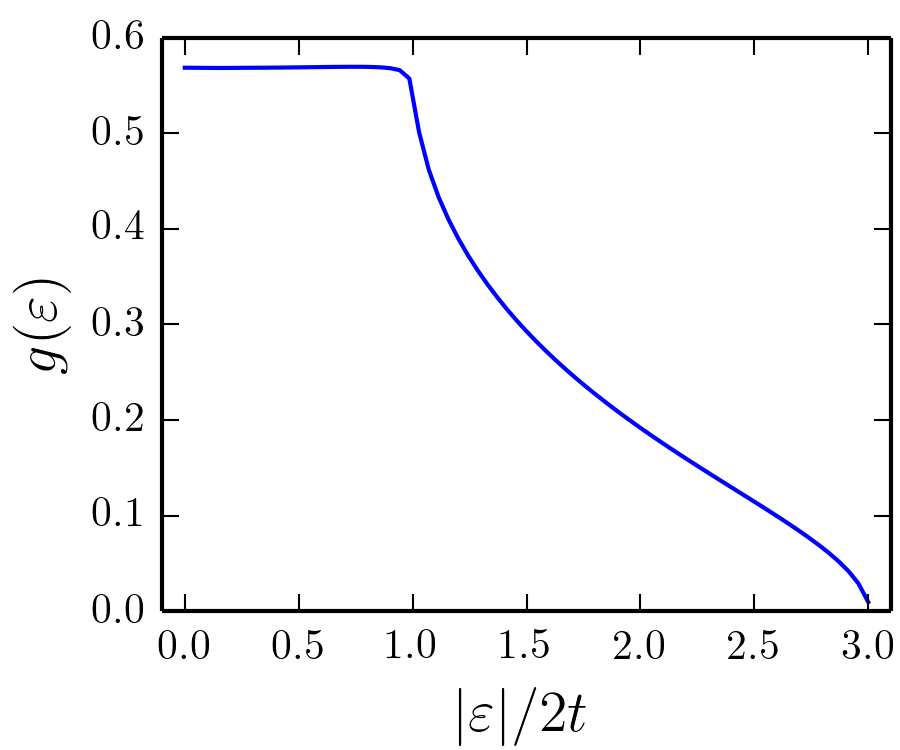
\includegraphics[width=0.5\textwidth]{figures/DOS_3D_tight-binding.png} \caption{
Density of states for the 3D tight-binding dispersion relation.  The zero of
energy has been chosen to be at the center of the band. }
\label{fig:g(E)tightbinding}
\end{figure}
This approach is cumbersome, and furthermore is limited because it only works
for non-interacting systems.   In our case we can take advantage of the results
of more sophisticated techniques that are at our disposal,  namely the
hight-temperature series expansion (HTSE) and the DQMC and NLCE solutions for
the thermodynamics of the Hubbard model.   All of these three methods provide
values of the density as a function of chemical potentia, from which the
compressibility is obtained as a first derivative.  

\subsection{Normalization of the compressibility} 

The results from the different thermodynamic treatments of the Hubbard model
give us the density (in units of $a^{-3}$) as a function of  $\mu/t$, the ratio
of the chemical potential to the tunneling energy.  We use $n'$ to represent
the density in units of $a^{-3}$,  $n'\equiv n a^{3}$.   We have for the
isothermal compressibility:
\begin{equation} 
\begin{split} 
  \kappa_{T}( n' )  &  =   \frac{1}{n^{2}} \frac{ \partial n }{ \partial \mu}  \\
    &   = - \frac{ \partial ( 1/n') } { \partial ( \mu/t ) }  \frac {a^{3}}{ t } 
\end{split}
\end{equation}
from where we can get the unitless quantity
\begin{equation} 
   \kappa_{T}(n') \frac{t }{ a^{3}} =  
    - \frac{ \partial ( 1/n') } { \partial ( \mu/t ) }
\end{equation}

To normalize this quantity we propose using the $T=0$ compressibility for a
non-interacting free fermion gas, multiplied by the tunneling matrix element
in the limit of zero lattice depth: 
\begin{equation}
  t(V_{0} \rightarrow 0\,E_{r} ) ~ \equiv t_{0} ~ = ~ 
   \frac{2}{\pi^{2}} E_{r} ~  =  ~ 0.203 \, E_{r} 
\end{equation} 
\begin{equation}
\begin{split} 
 \mathrm{Normalization:} ~~~~ 
   \kappa_{T}^{0}(n') \frac{t_{0}}{a^{3}}  & = 
   \frac{1}{ (n')^{5/3}}  \frac{ 3 s^{2/3} }{ (6\pi^{2})^{2/3}} 
   \frac{\pi^{2}}{2}  \frac{ t_{0}}{E_{r}}  \\ 
  & =  \frac{1}{ (n')^{5/3}}  \frac{ 3 s^{2/3} }{ (6\pi^{2})^{2/3}} 
\end{split} 
\end{equation}

We define the normalized compressibility $\kappa'$ as 
\begin{equation} 
 \kappa'(n') = \frac{ \kappa_{T}(n') \, t }{ \kappa_{T}^{0}(n') \, t_{0} } 
\end{equation} 
and obtain
\begin{equation}
\begin{split}
 \kappa'(n') &  = - \frac{ \partial (1/n') }{ \partial (\mu/t)}
   n'^{5/3}\frac{  (6\pi^{2})^{2/3} }{ 3s^{2/3} } \\
    & =  \frac{1}{n'^{1/3}} \frac{ \partial n' }{\partial(\mu/t)}  
         \frac{  (6\pi^{2})^{2/3} }{ 3s^{2/3} } \\
         &  =  \frac{ \partial ( n'^{2/3} ) }{ \partial (\mu/t) } 
    \frac{3}{2} 
         \frac{  (6\pi^{2})^{2/3} }{ 3s^{2/3} } \\
         &  =  \frac{ \partial ( n'^{2/3} ) }{ \partial (\mu/t) } 
         \frac{  (6\pi^{2})^{2/3} }{ 2s^{2/3} } \\
         &  =  4.79 \frac{ \partial ( n'^{2/3} ) }{ \partial (\mu/t) } \\ 
         &  =  4.79 \frac{ \partial ( n'^{2/3} ) }{\partial r} 
         \frac{ \partial r }{ \partial (\mu/t) } \\
         &  =  4.79 \frac{ \partial ( n'^{2/3} ) }{\partial r} 
         \left( \frac{ \partial (\mu/t) }{ \partial r } \right)^{-1} \\
\end{split}
\end{equation} 
    




 

\bibliographystyle{osa} 
\bibliography{kappa}

\end{document}




